\documentclass[A4,12PT, english, twocolumn]{journal}
\usepackage{amsmath,amssymb,amsfonts}
\usepackage[margin=0.7in]{geometry}
\usepackage{graphicx}
\usepackage{enumitem}
\usepackage{xcolor}
\usepackage{hyperref}
\usepackage{tabularray}
\usepackage{multicol}
\usepackage{tikz}
\usepackage{circuitikz}
\usepackage{scalerel}
\usepackage{pict2e}
\usepackage{tkz-euclide}
\usetikzlibrary{calc}
\usetikzlibrary{patterns,arrows.meta}
\usetikzlibrary{shadows}
\usetikzlibrary{external}

%pgfplots
\usepackage{pgfplots}
\pgfplotsset{compat=newest}
\usepgfplotslibrary{statistics}
\usepgfplotslibrary{fillbetween}

\def\infinity{\rotatebox{90}{8}}

% Hiperlink
\hypersetup{
    colorlinks=true,
    linkcolor=blue,
    filecolor=magenta,      
    urlcolor=cyan,
    pdftitle={Overleaf Example},
    pdfpagemode=FullScreen,
}
%\usepackage{style}
\NewDocumentCommand{\Log}{o}{%
\IfNoValueTF{#1}{}{{}^{#1}\!}\log}%
  
%command buat logaritma dengan basisnya di pojok kiri
%\textheight=17cm
%\textwidth=10cm
%\usepackage{blindtext}
\setenumerate[1]{itemsep=0,5cm}
\setenumerate[2]{topsep=5pt, itemsep=5pt, label=\textbf{\Alph*}.}

\title{Matematika Saintek \& Fisika UTUL UGM 2017 Kode 713}
\author{Fauzan Akbar Sukandar Putra \\ \LaTeX}

\begin{document}
\maketitle

%\begin{minipage}{0.5\textwidth}
\begin{enumerate}

%1%
\item Jika ${}^3 \log x + {}^4 \log y^2 = 5$, maka nilai maksimum dari ${}^3 \Log x \cdot {}^2 \Log y$ adalah \dots
    \begin{enumerate}
        \item $\frac{25}{4}$
        \item $\frac{25}{9}$
        \item $\frac{25}{16}$
        \item $1$
        \item $\frac{25}{36}$
    \end{enumerate}

%2%
\item Dalam pemilihan pengurus kelas, terpilih $5$ calon, $3$ laki-laki dan $2$ perempuan. Posisi yang tersedia yaitu ketua, wakil ketua, sekretaris, bendahara I, dan bendahara II. Jika ketua kelas harus laki-laki, maka banyaknya susunan pengurus yang mungkin adalah \dots
    \begin{enumerate}
        \item $5$
        \item $24$
        \item $48$
        \item $72$
        \item $120$
    \end{enumerate}

%3%
\item Diketahui $f(0)=1$ dan $f'(0)=2$. Jika $g(x)= \frac{1}{\left(2f(x)-1 \right)^3}$, maka $g'(0)=$ \dots
    \begin{enumerate}
        \item $-12$
        \item $-6$
        \item $6$
        \item $8$
        \item $11$
    \end{enumerate}

%4%
\item Jika akar-akar persamaan suku banyak $x^3-12x^2+(p+4)x-(p+8)=0$ membentuk deret aritmatika dengan beda $2$, maka $p-36=$ \dots
    \begin{enumerate}
        \item $-2$
        \item $0$
        \item $4$
        \item $8$
        \item $12$
    \end{enumerate}

%5%
\item Titik pusat lingkaran $L$ terletak di kuadran satu dan terletak pada garis $y=2x+1$. Jika lingkaran $L$ menyinggung sumbu $Y$ di titik $(0,11)$, maka persamaan lingkaran $L$ adalah \dots
    \begin{enumerate}
        \item $x^2+y^2-5x-11y=0$
        \item $x^2+y^2+5x+11y-242=0$
        \item $x^2+y^2-10x-22y+121=0$
        \item $x^2+y^2-5x+11y=0$
        \item $x^2+y^2+10x+22y-363=0$
    \end{enumerate}

%6%
\item Jika daerah yang dibatasi oleh kurva $y=x^2$ dan garis $y=(2m-2)x$ mempunyai luas $1\frac{1}{3}$, maka $m=$ \dots
    \begin{enumerate}
        \item $2\frac{1}{2}$ atau $-\frac{1}{2}$
        \item $2$ atau $0$
        \item $3\frac{1}{2}$ atau $-1\frac{1}{2}$
        \item $4$ atau $-2$
        \item $4\frac{1}{2}$ atau $-2\frac{1}{2}$
    \end{enumerate}

%7%
\item Jika tiga bilangan berbeda $x, \; y,$ dan $z$ membentuk barisan geometri, maka $\frac{1}{x-y}- \frac{1}{y-z}=$ \dots
    \begin{enumerate}
        \item $\frac{1}{x}$
        \item $-\frac{1}{y}$
        \item $\frac{1}{z}$
        \item $\frac{1}{x+z}$
        \item $\frac{1}{x-z}$
    \end{enumerate}

%8%
\item Semua nilai $x$ yang memenuhi $\sqrt{x^2-7x+6} \geq 2x$ adalah \dots
    \begin{enumerate}
        \item $\left\{ x \in \mathbb{R} \left|\right. -3 \leq x \leq \frac{1}{3} \right\}$
        \item $\left\{ x \in \mathbb{R} \left|\right. -3 \leq x \leq \frac{2}{3} \right\}$
        \item $\left\{ x \in \mathbb{R} \left|\right. x \leq -3 \right.$ atau $\left. x \geq \frac{2}{3} \right\}$
        \item $\left\{ x \in \mathbb{R} \left|\right. x \leq 1 \right.$ atau $\left. x \geq 6 \right\}$
        \item $\left\{ x \in \mathbb{R} \left|\right. x \leq \frac{2}{3} \right\}$
    \end{enumerate}

%9%
\item $\lim\limits_{x \longrightarrow -4} \dfrac{1- \cos{(x+4)}}{x^2+8x+16}=$ \dots
    \begin{enumerate}
        \item $-2$
        \item $-\frac{1}{2}$
        \item $\frac{1}{3}$
        \item $\frac{1}{2}$
        \item $2$
    \end{enumerate}

%10%
\item Himpunan penyelesaian pertidaksamaan
\begin{center}
    $^\frac{1}{2}\Log{(2x-1)} + ^\frac{1}{2}\Log{(2-x)} \geq 2 \; ^\frac{1}{2}\Log{x}$
\end{center}
adalah \dots
    \begin{enumerate}
        \item $\left\{ x \in \mathbb{R} \left|\right. \frac{2}{3} \leq x \leq 1 \right\}$
        \item $\left\{ x \in \mathbb{R} \left|\right. x \leq \frac{2}{3} \right.$ atau $\left. x \geq 1 \right\}$
        \item $\left\{ x \in \mathbb{R} \left|\right. \frac{1}{2}<x \leq \frac{2}{3} \right.$ atau $\left. 1 \leq x <2 \right\}$
        \item $\left\{ x \in \mathbb{R} \left|\right. \frac{1}{2} \leq x \leq \frac{2}{3} \right.$ atau $\left. 1 \leq x \leq 2 \right\}$
        \item $\left\{ x \in \mathbb{R} \left|\right. x \lwq \frac{1}{2} \right.$ atau $\left. x>2 \right\}$
    \end{enumerate}

%11%
\item Jika panjang vektor $\Vec{u}, \Vec{v},$ dan $(\Vec{u}+\Vec{v})$ berturut-turut $12, \; 8,$ dan $4\sqrt{7}$. Maka besar sudut antara $\Vec{u}$ dan $\Vec{v}$ adalah \dots
    \begin{enumerate}
        \item $45^\circ$
        \item $60^\circ$
        \item $90^\circ$
        \item $120^\circ$
        \item $150^\circ$
    \end{enumerate}

%12%
\item Jika proyeksi $\Vec{u}= (6,1)$ pada $\Vec{p}= (1,1)$ sama dengan proyeksi $\Vec{v}= (\alpha, -5)$ pada $\Vec{p}$, maka nilai $\alpha$ yang memenuhi adalah \dots
    \begin{enumerate}
        \item $-12$
        \item $-2$
        \item $2$
        \item $5$
        \item $12$
    \end{enumerate}

%13%
\item Misalkan $x_1$ dan $x_2$ merupakan akar-akar persamaan $px^2+qx-1=0$, $p \neq 0$. Jika $\frac{1}{x_1}+\frac{1}{x_2}=-1$ dan $x_1=-\frac{3}{2}x_2$, maka $p+q=$ \dots
    \begin{enumerate}
        \item $-7$
        \item $-5$
        \item $0$
        \item $5$
        \item $7$
    \end{enumerate}

%14%
\item Diketahui kubus $ABCDEFGH$. Jika $\alpha$ adalah sudut antara bidang $AHF$ dan $CHF$, maka $\sin{\alpha}=$ \dots
    \begin{enumerate}
        \item $-\frac{2}{3}\sqrt{2}$
        \item $-\frac{1}{3}\sqrt{2}$
        \item $\frac{1}{3}$
        \item $\frac{1}{3}\sqrt{2}$
        \item $\frac{2}{3}\sqrt{2}$
    \end{enumerate}

%15%
\item Deketahui $0 \leq x < \frac{\pi}{2}$. Jika
\begin{center}
    $5 \sin{2x}+10 \cos^2{x}=26 \cos{2x}$,
\end{center}
maka $\cos{2x}=$ \dots
    \begin{enumerate}
        \item $\frac{215}{233}$
        \item $\frac{205}{233}$
        \item $\frac{169}{233}$
        \item $\frac{115}{233}$
        \item $\frac{105}{233}$
    \end{enumerate}
    
    
%FISIKA %
%16%
\newpage
\item Sebuah partikel bergerak dalam satu dimensi dimana hubungan antara kecepatan $v$ dengan jarak $x$ dinyatakan sebagai
\begin{center}
    $x=at^2-bt$ dan $y=ct+d$
\end{center}
dengan $a, \; b, \; c,$ dan $d$ adalah konstanta positif. Lintasan partikel tersebut dalam bidang $xy$ berbentuk \dots
    \begin{enumerate}
        \item Garis lurus
        \item Lingkaran
        \item Elips
        \item Parabola
        \item Hiperbola
    \end{enumerate}
  
%17%
\item Sebuah partikel bermassa $m$ bergerak pada lintasan lingkaran horizontal berjari-jari $r$ diatas meja kasar. Partikel itu terikat pada tali tepat pada pusat lingkaran. Kelajuan partikel mula-mula $v_0$. Setelah menyelesaikan satu lingkaran penuh, kelajuan partikel berkurang menjadi $\frac{1}{2} v_0$. Hitunglah usaha yang dilakukan pada gesekan selama satu putaran tersebut dinyatakan dalam $m, \; v_0,$ dan $r.$
    \begin{enumerate}
        \item $- \frac{1}{2} mv_0^2$
        \item $- \frac{3}{4} mv_0^2$
        \item $-\frac{1}{2} \left(\frac{1}{2} mv_0^2 \right)$
        \item $-\frac{3}{4} \left(\frac{1}{2} mv_0^2 \right)$
        \item $\frac{1}{2} mv_0^2$
    \end{enumerate}
     
%18%
\item Pada sistem seperti yang ditunjukkan dengan gambar, diketahui $m_1 =8 \; kg, \; m_2=10 \; kg,$ koefisien gesekan statik antara $m_2$ dengan alas meja adalah $\mu_s = 0,3$. Kedua katrol tidak bermassa, serta tali juga tidak bermassa. Agar sistem dalam keadaan diam, rentang massa $m_3$ adalah \dots
\begin{center}
    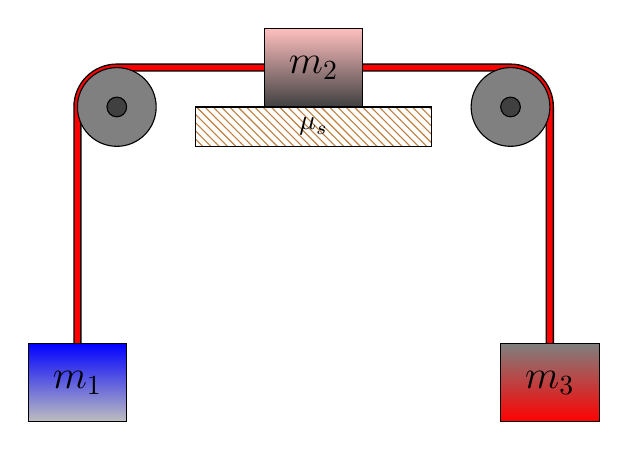
\begin{tikzpicture}[scale=0.5]
        %GRID
        %\draw[lightgray] (0,0) grid (8,15);
        
        %KOORDINAT
        \coordinate (A) at (2,4);
        \coordinate (B) at (12,4);
        
        %TALI
        \draw[line width=3pt, black] (1,-2) -- (1,4)  arc (180:90:1cm) -- (12,5) arc (90:0:1cm) -- (13,-2);
        
        \draw[line width=2pt, red] (1,-2) -- (1,4)  arc (180:90:1cm) -- (12,5) arc (90:0:1cm) -- (13,-2);
        
        %KATROL
        \draw[fill=gray] (A) circle (1cm);
        \draw[fill=darkgray] (A) circle (0.25cm);
        
        \draw[fill=gray] (B) circle (1cm);
        \draw[fill=darkgray] (B) circle (0.25cm);
        
        %BALOK
        \shadedraw[top color=pink, bottom color=darkgray] (5.75,4) rectangle node[midway]{\Large $m_2$} (8.25,6);

        \shadedraw[top color=blue, bottom color=lightgray] (-0.25,-4) rectangle node[midway]{\Large $m_1$} (2.25,-2);

        \shadedraw[top color=gray, bottom color=red] (11.75,-4) rectangle node [midway]{\Large $m_3$} (14.25,-2);
        
        %MEJA
        \filldraw[pattern=north west lines, pattern color=brown] (4,3) rectangle node[midway]{\Lage $\mu_s$}(10,4);
        
    \end{tikzpicture}
\end{center}
    \begin{enumerate}
        \item $6 \to 12 \; kg$
        \item $7 \to 11 \; kg$
        \item $5 \to 13 \; kg$
        \item $6 \to 13 \; kg$
        \item $5 \to 11 \; kg$
    \end{enumerate}
   
%19% 
\item Seseorang yang memiliki berat $W$ berada pada suatu elevator. Jika elevator dipercepat ke atas, gaya yang diderita elevator adalah $N_1$, sedangkan jika elevator dipercepat ke bawah dengan besar percepatan yang sama, gaya pada alas elevator adalah $N_2$. Perbandingan antara percepatan elevator dengan $g$ dapat dituliskan sebagai \dots
    \begin{enumerate}
        \item $\frac{N_1-N_2}{2W}$
        \item $\frac{N_2-N_1}{2W}$
        \item $\frac{N_1-N_2}{W}$
        \item $\frac{N_1+N_2}{2W}$
        \item $\frac{N_1+N_2}{W}$
    \end{enumerate}

%20%
\item Sebuah bola bermassa $m$ menumbuk bola bermassa $2m$ yang diam secara lenting sempurna. Besarnya energi kinetik dari bola $m$ yang hilang setelah tumbukan dibagi dengan energi kinetiknya sebelum tumbukan adalah \dots
    \begin{enumerate}
        \item $\frac{1}{2}$
        \item $\frac{5}{9}$
        \item $\frac{6}{9}$
        \item $\frac{7}{9}$
        \item $\frac{8}{9}$
    \end{enumerate}

%21%
\item Selembar kertas bermassa $m$ berada di atas meja. Diatas kertas diletakkan balok bermassa $M$. Koefisien gesek statik dan kinetik antara kertas dan balok adalah $\mu_{s1}$ dan $\mu_{k1}$ berturutan. Sedangkan koefisien gesek statik dan kinetik antara kertas dan meja adalah $\mu_{s2}$ dan $\mu_{k2}$ berturutan. Besar gaya minimum yang harus diberikan untuk menarik kertas dari bawah balok tanpa membawa serta balok adalah \dots
    \begin{enumerate}
        \item $Mg(\mu_{s1}+\mu_{k2})+mg \mu_{k2}$
        \item $Mg\mu_{s1}+mg\mu_{s2}$
        \item $Mg(\mu_{s1}+\mu_{s2})+mg \mu_{s2}$
        \item $Mg\mu_{s2}+mg\mu_{s2}$
        \item $(M+m)g(\mu_{s1}+\mu_{s2})$
    \end{enumerate}
    
%22% 
\item Pada dawai piano dengan panjang $L$ dan massa $m$, besarnya tegangan pada dawai agar menghasilkan frekuensi nada atas pertama $f$ adalah \dots
    \begin{enumerate}
        \item $4mLf^2$
        \item $mLf^2$
        \item $\frac{4}{9} mLf^2$
        \item $\frac{1}{4} mLf^2$
        \item $\frac{4}{25} mLf^2$
    \end{enumerate}
    
%23%
\item Jika periode bandul sederhana bergantung pada panjang bandul $L$ dan percepatan gravitasi $g$ dengan dimensi $\frac{L}{T^2}$, manakah ungkapan periode bandul sederhana yang benar dengan $k$ adalah sebuah tetapan?
    \begin{enumerate}
        \item $T=k \sqrt{\frac{L}{g}}$
        \item $T=k \sqrt{Lg}$
        \item $T=k \sqrt{\frac{g}{L}}$
        \item $T=k \sqrt{Lg}$
        \item $T=kLg$
    \end{enumerate}
    
%24%  
\item Didepan sebuah cermin cekung diletakkan objek pada jarak $10 \; cm$ dari cermin. Ternyata bayangan yang terbentuk nyata dan terbalik, serta berada di jarak yang sama dengan bendanya. Radius kelengkungan cermin ini adalah \dots cm
	\begin{enumerate}
		\item $10$
		\item $7,5$
		\item $5,0$
		\item $2,5$
		\item $1,25$
	\end{enumerate}
	
%25%
\item Sebuah proton masuk ke daerah yang bermedan magnet dan bermedan listrik dengan kecepatan awal konstan. Arah medan magnet searah dengan arah medan istrik. Bila kecepatan proton awalnya searah dengan arah medan listrik, maka proton akan \dots
   \begin{enumerate}
        \item Bergerak lurus dengan kecepatan konstan
        \item Bergerak lurus diperlambat
        \item Bergerak lurus dipercepat
        \item Bergerak dalam lintasan melengkung
        \item Diam
   \end{enumerate}
   
%26%
\item Terdapat tiga kapasitor $40 \; \mu F, 60 \; \mu F,$ dan $120 \; \mu F$ yang akan disusun sedemikian rupa sehingga menghasilkan resultan kapasitansi sebesar $80 \; \mu F$. Susunan yang benar adalah \dots
    \begin{enumerate}
        \item
            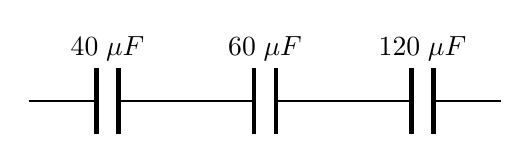
\begin{tikzpicture}[baseline]
                \draw[thick] (0,0) to[capacitor, a^=$40\; \mu F$] (2,0) to[capacitor, a^=$60\; \mu F$] (4,0) to[capacitor, a^=$120\; \mu F$] (6,0);
            \end{tikzpicture}
        \item 
            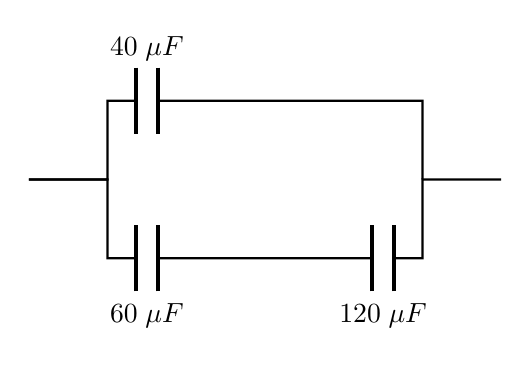
\begin{tikzpicture}[baseline]
                \draw[thick] (0,0) -- (1,0) -- (1,1) to[capacitor, a^=$40\; \mu F$] (2,1) -- (5,1) -- (5,0);
                \draw[thick] (6,0) -- (5,0) -- (5,-1) to[capacitor, a^=$120\; \mu F$] (4,-1) -- (2,-1) to[capacitor, a^=$60\; \mu F$] (1,-1) -- (1,0) -- (0,0);
            \end{tikzpicture}
        \item 
            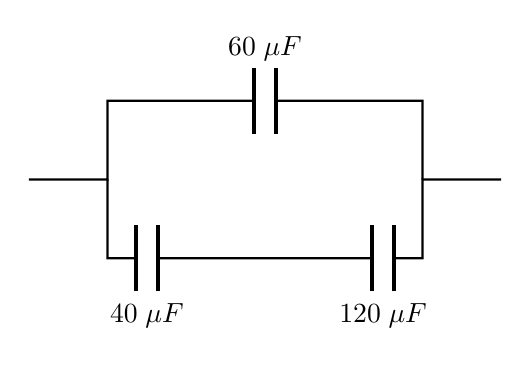
\begin{tikzpicture}[baseline]
                \draw[thick] (0,0) -- (1,0) -- (1,1) to[capacitor, a^=$60\; \mu F$] (5,1) -- (5,0);
                \draw[thick] (6,0) -- (5,0) -- (5,-1) to[capacitor, a^=$120\; \mu F$] (4,-1) -- (2,-1) to[capacitor, a^=$40\; \mu F$] (1,-1) -- (1,0);
            \end{tikzpicture}
        \item 
             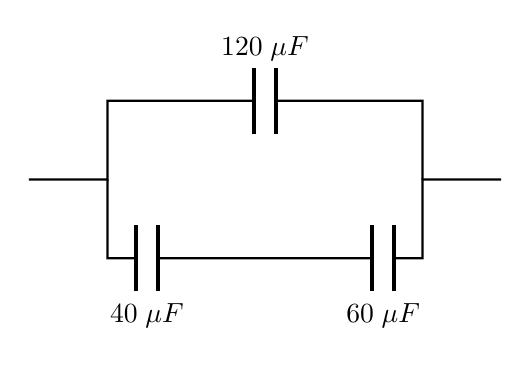
\begin{tikzpicture}[baseline]
                \draw[thick] (0,0) -- (1,0) -- (1,1) to[capacitor, a^=$120\; \mu F$] (5,1) -- (5,0);
                \draw[thick] (6,0) -- (5,0) -- (5,-1) to[capacitor, a^=$60\; \mu F$] (4,-1) -- (2,-1) to[capacitor, a^=$40\; \mu F$] (1,-1) -- (1,0);
            \end{tikzpicture}
        \item 
            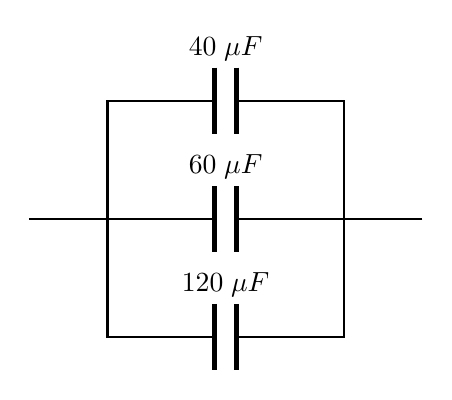
\begin{tikzpicture}[baseline]
                \draw[thick] (0,0) -- (1,0) -- (1,1.5) to[capacitor, a^=$40\; \mu F$] (4,1.5) -- (4,0);
                \draw[thick] (5,0) -- (4,0) to[capacitor, a=$60\; \mu F$] (1,0);
                \draw[thick] (1,0) -- (1,-1.5) to[capacitor, a^=$120\; \mu F$] (4,-1.5) -- (4,0);
            \end{tikzpicture}
    \end{enumerate}
  
%27%  
\item Dua buah muatan $q \; (+2 \times 10^{-6} coulomb)$ terpisah sejauh $d \; (2 \; cm)$ sebagaimana ditunjukkan pada gambar. Hitunglah potensial listrik di titik $C$.
\begin{center}
    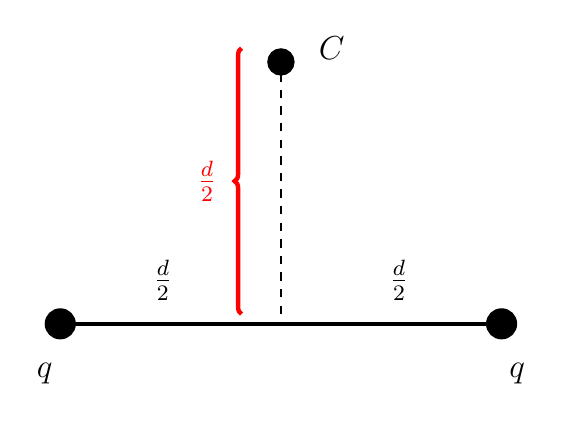
\begin{tikzpicture}
        \draw[white] (0,0) -- node[midway, black, above=5pt]{\large $\frac{d}{2}$} (3,0);
        \draw[white] (3,0) -- node[midway, black, above=5pt]{\large $\frac{d}{2}$} (6,0);
        %GARIS HORIZONTAL
        \draw[{Circle[scale=1.5]}-{Circle[scale=1.5]}, ultra thick] (0,0) node[below=10pt]{\large $q$} -- (6,0) node[below=10pt]{\large $q$};
        %BRACKETS
        \draw [decorate, decoration = {brace}, ultra thick, red] (2.5,0.125) --  (2.5,3.5) node[midway, left=5pt]{\large $\frac{d}{2}$};
        %GARIS VERTIKAL
        \draw[thick, dashed, -{Circle[scale=2]}] (3,0.125) -- (3,3.5) node[right=10pt]{\large $C$};
    \end{tikzpicture}
\end{center}
    \begin{enumerate}
        \item $3,25 \times 10^6 \; V$
        \item $2,57 \times 10^6 \; V$
        \item $3,25 \times 10^5 \; V$
        \item $2,57 \times 10^5 \; V$
        \item $0 \; V$
    \end{enumerate}
    
%28%  
\item Sebuah termometer $X$ akan dikalibrasi dengan termometer Fahrenheit $(F)$. Pada suhu $80^\circ \; F$, termometer $X$ menunjukkan angka $95^\circ \; X$. Sedangkan pada suhu $120^\circ \; F$, termometer $X$ menunjukkan angka $125^\circ \; X$. Jika diasumsikan kedua termometer tersebut memiliki hubungan suhu yang linear, maka pada saat kedua termometer tersebut menunjukkan angka yang sama, angka yang ditunjukkan termometer Celcius adalah \dots
    \begin{enumerate}
        \item $60^\circ \; C$
        \item $72^\circ \; C$
        \item $80^\circ \; C$
        \item $85^\circ \; C$
        \item $90^\circ \; C$
    \end{enumerate}

%29%  
\item Dua benda $m$ dan $M$ terpisah dengan jarak yang sangat jauh, kemudian bergerak saling mendekati karena gaya gravitasi. Pada saat jarak antara keduanya adalah $d$, besarnya kecepatan relatif antara keduanya adalah \dots \\
\textbf{($G=$ konstanta gravitasi universal)}
    \begin{enumerate}
        \item $\sqrt{\frac{2G(M-m)}{d}}$
        \item $\sqrt{\frac{2G(M+m)}{d}}$
        \item $\sqrt{\frac{2GMm}{(M+m)d}}$
        \item $\sqrt{\frac{G(M+m)}{d}}$
        \item $\sqrt{\frac{GMm}{(M+m)d}}$
    \end{enumerate}

%30%
\item Fungsi kerja logam $A$ dua kali fungsi kerja logam $B$. Hal ini bererti \dots
    \begin{enumerate}
        \item Frekuensi minimal berkas cahaya untuk terjadinya efek fotolistrik pada logam $A$ dua kalinya frekuensi minimal terjadinya efek fotolistrik pada logam $B$
        \item Frekuensi minimal berkas cahaya untuk terjadinya efek fotolistrik pada logam $B$ dua kalinya frekuensi minimal terjadinya efek fotolistrik pada logam $A$
        \item Akibat foton dengan frekuensi yang sama, energi kinetik elektron yang lepas dari logam $A$ dua kali energi kinetik elektron yang lepas dari logam $B$
        \item Akibat foton dengan frekuensi yang sama, energi kinetik elektron yang lepas dari logam $B$ dua kali energi kinetik elektron yang lepas dari logam $A$
        \item Akibat foton dengan frekuensi yang sama, energi kinetik elektron yang lepas dari logam $A$ sama dengan energi kinetik elektron yang lepas dari logam $B$
    \end{enumerate}
 
%31%
\item Setelah tiga jam. Sebanyak $93,75\%$ zat radioaktif $X$ telah meluruh menjadi zat lain. Waktu paruh zat $X$ adalah \dots
    \begin{enumerate}
        \item $30$ menit
        \item $36$ menit
        \item $45$ menit
        \item $60$ menit
        \item $90$ menit
    \end{enumerate}

%32%
\item Sebuah elektron bergerak dalam medan listrik seragam $1,0 \times 10^6 \; N/C$. Jika mula-mula elektron tersebut diam, hitunglah waktu yang ditempuh elektron agar kecepatannya menjadi $1/10$ kecepatan cahaya \dots 
    \begin{enumerate}
        \item $1,67 \times 10^{-10} \; s$
        \item $1,67 \times 10^{-9} \; s$
        \item $1,67 \times 10^{-8} \; s$
        \item $1,67 \times 10^{-7} \; s$
        \item $1,67 \times 10^{-6} \; s$
    \end{enumerate}

%33%
\item Sebuah foton memiliki panjang gelombang yang sama dengan panjang gelombang de Broglie sebuah elektron. Jika $c=$ laju cahaya dalam vakum, $E_0=$ energi diam elektron dan $p_e$ adalah momentum elektron, perbandingan antara energi foton dengan energi kinetik elektron non-relativisstik adalah \dots
    \begin{enumerate}
        \item $\frac{E_0}{p_ec}$
        \item $\frac{2E_0}{p_ec}$
        \item $\frac{p_ec}{2E_0}$
        \item $\frac{p_ec}{E_0}$
        \item $\frac{2p_ec}{E_0}$
    \end{enumerate}

%34%
\item Sebuah elips memiliki setengah sumbu panjang $a$ dan setengah sumbu pendek $b$ jika diukur dalam keadaan diam. Seorang pengamat bergerak sepanjang garis lurus melalui pusat elips tegak lurus bidang elips dengan kecepatan $v$. Luas elips itu menurut pengamat yang bergerak adalah \dots
    \begin{enumerate}
        \item $\pi ab$
        \item $\pi ab \sqrt{1- \left(\frac{v}{c} \right)^2}$
        \item $\pi ab \left(1- \left(\frac{v}{c} \right)^2 \right)$
        \item $\pi ab \left(1- \left(\frac{v}{c} \right)^2 \right)^{-\frac{1}{2}}$
        \item $\pi ab \left(1- \left(\frac{v}{c} \right)^2 \right)^{-1}$
    \end{enumerate}

%35%
\item Sebuah terowongan yang lurus digali pada planet berbentuk bola yang kerapatan massanya $\rho_0$ konstan. Terowongan itu melewati pusat planet dan tegak lurus terhadap sumbu rotasi planet, yang tetap dalam ruang. Planet berputar dengan kecepatan sudut $\omega$ sedemikian rupa sehingga benda-benda dalam terowongan tidak memiliki percepatan relatif terhadap terowongan. Hitunglah nilai $\omega$.
    \begin{enumerate}
        \item $\left( \frac{4}{3}G \pi \rho_0 \right)^{\frac{1}{2}}$
        \item $\left( \frac{2}{3}G \pi \rho_0 \right)^{\frac{1}{2}}$
        \item $\left( \frac{4}{3}G \pi \right)^{\frac{1}{2}} \rho_0$
        \item $\left( \frac{2}{3}G \pi \right)^{\frac{1}{2}} \rho_0$
        \item $\frac{1}{4}G \pi \rho_0^2$
    \end{enumerate}

\end{enumerate}
\end{document}  
